\documentclass[a4paper,11pt]{jsarticle}


% 数式
\usepackage{amsmath,amsfonts,amssymb}
\usepackage{empheq}
\usepackage{bm}
% 画像
\usepackage[dvipdfmx]{graphicx}
\usepackage[dvipdfmx]{color}
\usepackage{siunitx}
\usepackage{wrapfig}
\usepackage{cases}
\usepackage{dcolumn}
\makeatletter
\newcommand{\figcaption}[1]{\def\@captype{figure}\caption{#1}}
\newcommand{\tblcaption}[1]{\def\@captype{table}\caption{#1}}
\makeatother

\usepackage{listings,jvlisting}
\lstset{
basicstyle={\ttfamily},
identifierstyle={\small},
commentstyle={\smallitshape},
keywordstyle={\small\bfseries},
ndkeywordstyle={\small},
stringstyle={\small\ttfamily},
frame={tb},
breaklines=true,
columns=[l]{fullflexible},
numbers=left,
xrightmargin=0zw,
xleftmargin=3zw,
numberstyle={\scriptsize},
stepnumber=1,
numbersep=1zw,
lineskip=-0.5ex
}

\begin{document}

\title{各質点の位置が直線状で変化する剛体単振り子}
\author{平林広}
\date{\today}
\maketitle

\begin{figure}[h]
  \centering
  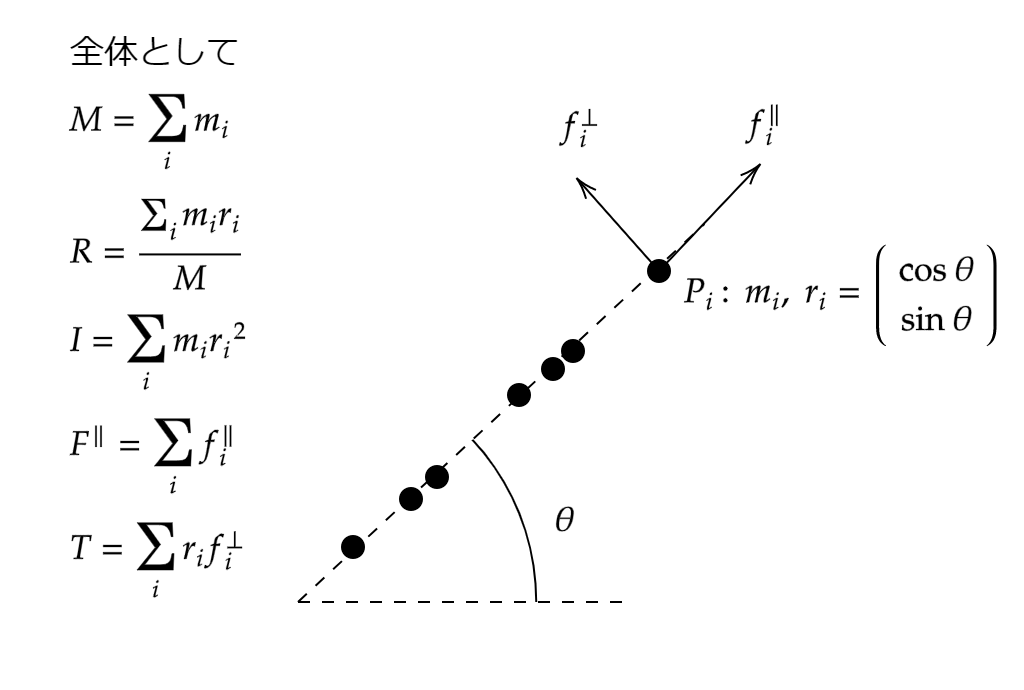
\includegraphics[width = 0.9\textwidth]{config.png}
  \caption{設定}
  \label{config.png}
\end{figure}

質点系$\{P_i\}$が一直線上に並ぶ剛体の単振り子の運動方程式を考える. 
ただし, 固定軸$\mathrm{O}$からの各質点の距離$\{r_i\}$は時間変化するものとする. 
結論としては
\begin{align*}
  \begin{cases}
  M \ddot{R} - M R \dot{\theta}^2 = F^\parallel
  \\
  \dot{I} \dot{\theta} + I \ddot{\theta} = T
  \end{cases}
\end{align*}
となる。

まず剛体全体としての全質量$M$, 
固定軸$\mathrm{O}$からの重心距離$R$, 
慣性モーメント$I$は
Fig. \ref{config.png}
の通りである。

$P_i$の固定軸$\mathrm{O}$を基準とした位置ベクトル$\mathrm{r}_i$は
\begin{align*}
  \mathrm{r_i} = r_i \begin{pmatrix}
    \cos \theta \\
    \sin \theta
  \end{pmatrix}
\end{align*}
だから、速度$\mathrm{v}_i$と加速度$\mathrm{a}_i$は
\begin{align*}
  \mathrm{v}_i = 
  \dot{r}_i \begin{pmatrix}
    \cos \theta \\
    \sin \theta
  \end{pmatrix}
  + r_i \dot{\theta} \begin{pmatrix}
    -\sin \theta \\
    \cos \theta
  \end{pmatrix},
\end{align*}
\begin{align*}
  \mathrm{a}_i = 
  \ddot{r}_i &\begin{pmatrix}
    \cos \theta \\
    \sin \theta
  \end{pmatrix}
  + \dot{r}_i \dot{\theta} \begin{pmatrix}
    -\sin \theta \\
    \cos \theta
  \end{pmatrix}
  \notag
  \\
  & + \dot{r}_i \dot{\theta} \begin{pmatrix}
    -\sin \theta \\
    \cos \theta
  \end{pmatrix}
  + r_i \ddot{\theta} \begin{pmatrix}
    -\sin \theta \\
    \cos \theta
  \end{pmatrix}
  + r_i \dot{\theta}^2 \begin{pmatrix}
    -\cos \theta \\
    -\sin \theta
  \end{pmatrix}
\end{align*}
と表される.
ニュートンの運動方程式
\begin{align*}
  m_i \mathrm{a}_i = 
  f_i^\parallel \begin{pmatrix}
    \cos \theta \\
    \sin \theta
  \end{pmatrix}
  + f_i^\perp \begin{pmatrix}
    -\sin \theta \\
    \cos \theta
  \end{pmatrix}
\end{align*}
と合わせて,
\begin{empheq}[left={\empheqlbrace}]{alignat=2}
  & m_i (\ddot{r}_i - r_i \dot{\theta}^2 ) = f_i^\parallel
  \label{newton_parallel}
  \\
  & m_i (2 \dot{r}_i \dot{\theta} + r_i \ddot{\theta} ) = f_i^\perp
  \label{newton_perp}
\end{empheq}
が分かる.

Equation \ref{newton_parallel} は添え字$i$について総和をとると
\begin{gather*}
  \sum_i m_i \ddot{r}_i - \sum_i m_i r_i \dot{\theta}^2 = \sum_i f_i^\parallel
  \\
  (\because M = \sum_i m_i, R = \frac{m_i r_i}{M}) \notag
  \\
  \Rightarrow M \ddot{R} - M R \dot{\theta}^2 = F^\parallel
\end{gather*}
が分かる。

Equation \ref{newton_perp}は少し難しい。
左辺が角運動量保存の式の手前であることが分かれば、両辺に$r_i$を書けることで
\begin{gather*}
  m_i (2 r_i \dot{r}_i \dot{\theta} + {r_i}^2 \ddot{\theta}) = r_i f_i^\perp
  \\
  \Rightarrow
  \frac{d}{dt} (m_i {r_i}^2 \dot{\theta} ) = r_i f_i^\perp
\end{gather*}
と各質点に置ける固定軸$\mathrm{O}$を基準として慣性モーメントが現れる。
添え字$i$について総和をとると
\begin{align*}
  \sum_i \frac{d}{dt} (m_i {r_i}^2 \dot{\theta} ) &= \sum_i r_i f_i^\perp
\end{align*}
ここで、$\sum$ と $\frac{d}{dt}$ が交換可能だと認めると
\begin{gather*}
  \frac{d}{dt} \left( \sum_i m_i {r_i}^2 \dot{\theta} \right) = \sum_i r_i f_i^\perp
  \\
  (\because I = \sum_i m_i {r_i}^2, T = \sum_i r_i f_i^\perp)
  \\
  \frac{d}{dt} \left( I \dot{\theta} \right) = T
  \\
  \dot{I} \dot{\theta} + I \ddot{\theta} = T
\end{gather*}
が分かる。

\end{document}